% SVN info for this file
\svnidlong
{$HeadURL$}
{$LastChangedDate$}
{$LastChangedRevision$}
{$LastChangedBy$}

\chapter{Il flusso del campo elettrico e la legge di Gauss}
\labelChapter{convergenzafunzioni}

\begin{introduction}
	‘‘Ecco una data importante nella storia della scienza: 5 novembre 1955. Fu il giorno in cui inventai il viaggio nel tempo. Me lo ricordo benissimo: stavo in piedi sul water attaccando un orologio, la porcellana era bagnata, sono scivolato e ho battuto la testa sul lavandino. Quando ho ripreso i sensi, ho avuto una rivelazione... una visione... un'immagine scolpita nella mente... un'immagine
	di questo. Questo rende possibile viaggiare nel tempo: il flusso canalizzatore!''
	\begin{flushright}
		\textsc{‘‘Doc'' Emmett L. Brown} a Marty McFly, \textit{Ritorno al futuro}.
	\end{flushright}
\end{introduction}
\lettrine[findent=1pt, nindent=0pt]{P}{er}  %TODO: intro
\section{Il flusso di un campo vettoriale}
\begin{define}[Flusso di un campo vettoriale]
\begin{minipage}{0.8\textwidth}
Il \textbf{flusso di un campo vettoriale attraverso una superficie orientata}\index{flusso di un campo vettoriale} $\Sigma$, parametrizzata da una funzione $\vba{r}(u,v)$, è
\begin{equation}
	\tcboxmath{\Phi_{\Sigma}(\vba{E})=\int_{\Sigma}\vba{E}\vdot\vbh{u}_nd\Sigma=\int_{\Sigma}\vba{E}\vdot\frac{\partial \vba{r}}{\partial u}\cross\frac{\partial \vba{r}}{\partial v}dudv}
\end{equation}
Matematicamente parlando, il flusso non è altro che un tipo di integrale superficiale di un campo vettoriale.%TODO: link ai richiami.\\
\end{minipage}\hspace{10pt}
\begin{minipage}{0.19\textwidth}
	\begin{center}
			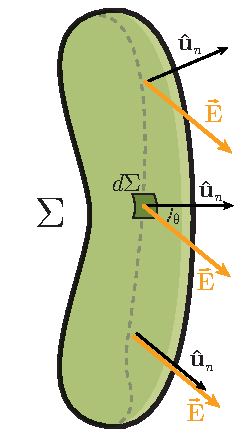
\includegraphics[width=0.6\textwidth]{images/chp2flusso.pdf}
	\end{center}
\end{minipage}
\end{define}
\begin{intuit}
	Se descriviamo la corrente di un fluido come l'acqua con un campo vettoriale $\vba{F}$, il flusso di $\vba{F}$ rappresenta \textit{quanto fluido} passa \textit{attraverso} una certa superficie per unità di tempo (anche se quest'ultima viene spesso sottintesa).\\
	Con questa interpretazione euristica si può capire anche perché l'integrale presenta nella definizione un \textit{prodotto scalare}: se l'acqua scorre perpendicolarmente alla superficie, molta acqua passerà e il flusso sarà dunque grande; al contrario, se il fluido scorre parallelamente alla superficie l'acqua non l'attraverserà mai e quindi il flusso è nullo. In altre parole, ciò che influisce sul flusso è la componente del flusso perpendicolare alla superficie!
\end{intuit}
\noindent Come abbiamo detto, la superficie deve essere \textbf{orientabile}: detto in una maniera suggestiva, intuitiva ma non formale come farebbero i fisici, una superficie con due \textit{facce distinte} e due \textit{orientazioni} possibili che corrispondono alla scelta di un \textit{campo normale} che punta sempre dalla parte di una delle facce.\\
In particolare, la superficie deve essere \textit{effettivamente orientata}, ossia si deve scegliere uno dei campi normali in modo da definire quando il flusso è positivo e quando è negativo. Generalmente, per convenzione si impone che il vettore normale alla superficie è orientato verso l'\textit{esterno}: quando la componente perpendicolare del campo vettoriale $\vba{E}$ e il vettore normale saranno \textit{concordi}, cioè quando $\vba{E}$ è \textit{uscente} dalla superficie, si ha un flusso \textit{positivo}; se il campo $\vba{E}$ è \textit{entrante} la superficie, allora si ha un flusso \textit{negativo}.
\begin{observe}%TODO: immagine?
	Data una superficie chiusa $\Sigma$, tracciamo una curva chiusa $\gamma$ su di essa; possiamo scindere $\Sigma$ in due sottosuperfici $\Sigma_1$ e $\Sigma_2$ che hanno in comune una superficie $\Sigma_{1,2}$ delimitata da $\gamma$.
	Il flusso per linearità di scinde in
	\begin{equation*}
		\Phi_{\Sigma}=\Phi_{\Sigma_1}+\Phi_{\Sigma_2}
	\end{equation*}
	In realtà, il flusso \textit{non} è influenzato da quale sia la superficie  $\Sigma_{1,2}$: infatti, per uno dei sottoflussi il contribuito dato da $ \Sigma_{1,2}$ sarà negativo perché il campo è entrante, ma per l'altro sottoflusso sarà positivo perché il campo è uscente.
	\begin{equation*}
		\Phi_{\Sigma}=\Phi_{\Sigma_1}+\Phi_{\Sigma_2}=\Phi_{\Sigma_1-\Sigma_{1,2}}+\Phi_{\Sigma_{1,2}}+\Phi_{\Sigma_2-\Sigma_{1,2}}-\Phi_{\Sigma_{1,2}}=\Phi_{\Sigma_1-\Sigma_{1,2}}+\Phi_{\Sigma_2-\Sigma_{1,2}}
	\end{equation*}
\end{observe}
\section{Legge di Gauss}
% https://mathinsight.org/surface_integral_vector_field_introduction4
% http://sites.science.oregonstate.edu/math/home/programs/undergrad/CalculusQuestStudyGuides/vcalc/flux/flux.html
% https://mathinsight.org/vector_field_fluid_flow
% https://tutorial.math.lamar.edu/classes/calciii/SurfIntVectorField.aspx
\begin{theorema}[Legge di Gauss]\index{legge!di Gauss}
	Il flusso del campo elettrostatico $\vba{E}$ attraverso un superficie \textbf{chiusa} è uguale alla somma algebrica (\textrm{o nel caso di una distribuzione continua}, dell'integrale) delle cariche contenute all'\textbf{interno} della superficie, comunque siano distribuite, divisa per $\epsilon_0$.
	\begin{itemize}
		\item \textbf{Caso discreto:}
		\begin{equation}
			\tcboxmath{\Phi_\Sigma(\vba{E})=\frac{\left(\sum_i q_i\right)_{int}}{\epsilon_0}}\label{LeggeGaussDiscreta}
		\end{equation}
		\item \textbf{Caso continuo:}
		\begin{equation}
			\tcboxmath{\Phi_\Sigma(\vba{E})=\frac{1}{\epsilon_0}\int_{V}\rho\left(x,y,z\right)dV\qquad\text{tale che}\ \partial V=\Sigma}\label{LeggeGaussContinua}
		\end{equation}
	\end{itemize}
\end{theorema}
Lo dimostreremo per una \textit{singola} carica contenuta nella superficie - dato che il caso per molteplici cariche e per una distribuzione continua seguono praticamente immediatamente - ma prima di farlo in modo formale, vediamo una derivazione più ‘‘fisica''.
\paragraph{Angolo solido}
Per far ciò, ci servirà la nozione di \textit{angolo solido}.
\begin{define}[Angolo solido]%\vspace{30pt}
	\begin{minipage}{0.6\textwidth}
		L'\textbf{angolo solido}\index{angolo solido} è una generalizzazione a tre dimensioni dell'angolo piano e dà una misura della parte di spazio compresa entro un fascio di semirette uscenti intorno ad un punto $P$.\\
		In termini matematici, esso è definito come l'area sulla \textit{sfera unitaria} intorno a $P$ individuata dalla superficie (finita) $\Sigma$:
		\begin{equation}
		\tcboxmath[colback=yellowpastellow!40!white,colframe=ceruleancrayola]{\Omega=\int d\Omega =\int \frac{d\Sigma_0}{r^2}=\int\frac{\cos\theta d\Sigma}{r^2}}
		\end{equation}
	\end{minipage}\hspace{5pt}
	\begin{minipage}{0.39\textwidth}
		\begin{center}
			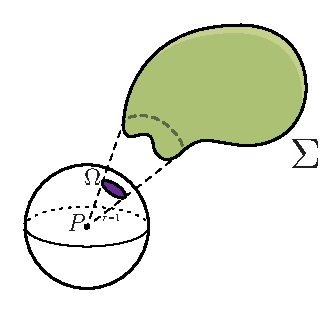
\includegraphics[width=1\textwidth]{images/chp2angolosolido.pdf}
		\end{center}
	\end{minipage}
dove
\begin{itemize}
	\item $d\Omega$ è l'angolo solido infinitesimo.
	\item $d\Sigma_0$ è la \textit{proiezione ortogonale} al raggio $r$ dell'elemento infinitesimo di superficie $d\Sigma$.
	\item $\theta$ è l'\textit{angolo polare} delle coordinate sferiche.
\end{itemize}
% https://tutorial.math.lamar.edu/classes/calciii/SurfIntVectorField.aspx
% https://betterexplained.com/articles/flux/
\end{define}
Poiché $d\Sigma_0$ è un elemento infinitesimo della calotta sferica, data una parametrizzazione in coordinate sferiche vale
\begin{equation*}
	d\Sigma_0=r^2\sin\theta d\theta d\phi
\end{equation*}
da cui segue che
\begin{equation}
	d\Sigma=\sin\theta d\theta d\phi
\end{equation}
Integrando $\theta$ da $0$ a $\pi$ e $\phi$ da $0$ a $2\pi$, si ottiene l'angolo solido sotto cui dal centro $P$ è vista tutta la superficie:
\begin{equation}
	\Omega=\int d\Omega=\int_0^{2\pi}d\phi\int_0^\pi d\theta\sin\theta=4\pi
\end{equation}
Questo risultato è valido per una qualunque superficie \textit{chiusa} che racchiuda $P$ - e ne corrisponde al valore massimo dell'angolo solido.\\
\begin{units}~\\
	\textbf{\textsc{Angolo solido:}} Steradiante  ($\unit{\steradian}$).\\
	\textit{Dimensioni:} $[\Omega]=\mathsf{1}$.
\end{units}
\paragraph{Derivazione fisica della legge di Gauss}
Dato il campo di Coulomb $\vba{E}$ generato dalla carica $q$, vogliamo determinare l'elemento di flusso infinitesimo $d\Phi(\vba{E})$, ossia il flusso tramite l'elemento d'area infinitesimo $d\Sigma$.
\begin{center}
	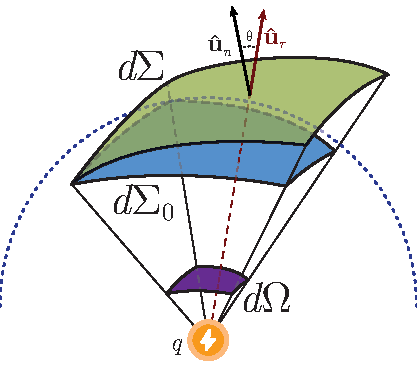
\includegraphics[width=0.36\textwidth]{images/chp2flussodim1.pdf}
\end{center}
Innanzitutto, si noti che l'angolo tra il versore radiale $\vbh{u}_r$ uscente dalla carica $q$ e il versore normale $\vbh{u}_n$ alla superficie coincide con un possibile angolo polare $\theta$ che parametrizza un punto della calotta sferica unitaria centrata in $q$.
\begin{equation*}
\vbh{u}_r\vdot\vbh{u}_n=\cos\theta
\end{equation*}
Il flusso infinitesimo diventa
\begin{equation*}
	d\Phi_{\Sigma}(\vba{E})=\vba{E}\vdot\vbh{u}_nd\Sigma=\frac{q}{4\pi\epsilon_0}\frac{\vbh{u}_r\vdot\vbh{u}_n}{r^2}d\Sigma=\frac{q}{4\pi\epsilon_0}\frac{\cos\theta}{r^2}d\Sigma=\frac{q}{4\pi\epsilon_0}\frac{d\Sigma_0}{r^2}=\frac{q}{4\pi\epsilon_0}d\Omega
\end{equation*}
\begin{observe}
	Il flusso del campo $\vba{E}$ generato da una carica puntiforme dipende solo dall'angolo solido e \textit{non} dalla superficie o dalla distanza dalla carica: il flusso è lo stesso per qualunque superficie il cui bordo si appoggi sul cono individuato dall'angolo solido.\\
	Questo è una \textit{diretta} conseguenza che il campo di Coulomb presenta un fattore $\nicefrac{1}{r^2}$; se la relazione fosse stata anche solo leggermente diversa non varrebbe tale dipendenza.
\end{observe}
Per una superficie (finita) e chiusa che racchiude la carica $q$ si ha
 \begin{equation*}
 	\Phi_\Sigma(\vba{E})=\frac{q}{4\pi\epsilon_0}\Omega=\frac{q}{\epsilon_0}
 \end{equation*}
\paragraph{Dimostrazione formale della legge di Gauss}
\begin{demonstration}
	Consideriamo inizialmente il caso con una carica sola. Per semplicità, poniamo l'origine del nostro sistema di riferimento dove è situata la carica. Data la simmetria di carattere radiale fornita dal campo elettrostatico di Coulomb, ci conviene utilizzare le coordinate sferiche
	\begin{equation*}
		\begin{cases}
			x=r\sin\theta\cos\phi\\
			y=r\sin\theta\sin\phi\\
			z=r\cos\theta
		\end{cases}
	\end{equation*}
	Parametrizziamo la superficie $\Sigma$ con l'angolo \textit{polare} $\theta$ e l'angolo \textit{azimutale} $\phi$ delle coordinate sferiche:
	\begin{align*}
		\vba{r}(\theta,\phi)&=x(\theta,\phi)\vba{u}_x+y(\theta,\phi)\vba{u}_y+z(\theta,\phi)\vba{u}_z=\\
		&=r(\theta,\phi)\sin\theta\cos\phi\vba{u}_x+r(\theta,\phi)\sin\theta\sin\phi\vba{u}_y+r(\theta,\phi)\cos\theta\vba{u}_z
	\end{align*}
	Osserviamo che per descrivere una superficie con le coordinate sferiche è necessario fornire la \textit{distanza} $r(\theta,\phi)$ dall'origine nella direzione indicata dagli angoli $\theta$ e $\phi$. Anzi, la parametrizzazione può essere espressa totalmente in termini \textit{radiali}! Infatti, il versore radiale è dato da
	\begin{equation*}
		\vbh{u}_r=\frac{\vbh{e}_r}{\abs{\vbh{e}_r}}=\frac{\pdv{x^i}{r}\vbh{u}_i}{1}=\sin\theta\cos\phi\vbh{u}_x+\sin\theta\sin\phi\vbh{u}_y+\cos\theta\vbh{u}_z
	\end{equation*}
	Raccogliendo $r(\theta,\phi)$ dalla parametrizzazione scritta prima si ottiene quindi
	\begin{equation*}
		\vba{r}(\theta,\phi)=r(\theta,\phi)\vbh{u}_r
	\end{equation*}
	Per definizione, il flusso è
	\begin{equation*}
		\Phi_{\Sigma}(\vba{E})=\int_{\Sigma}\vba{E}\vdot\vbh{u}_nd\Sigma=\int_{\Sigma}\vba{E}\vdot\vbh{u}_n\abs{\pdv{\vba{r}(\theta,\phi)}{\theta}\cross\pdv{\vba{r}(\theta,\phi)}{\phi}}d\theta d\phi\squarequal
	\end{equation*}
	Poiché il versore normale è
	\begin{equation*}
		\vbh{u}_n=\frac{\pdv{\vba{r}(\theta,\phi)}{\theta}\cross\pdv{\vba{r}(\theta,\phi)}{\phi}}{\abs{\pdv{\vba{r}(\theta,\phi)}{\theta}\cross\pdv{\vba{r}(\theta,\phi)}{\phi}}}
	\end{equation*}
	il flusso si può calcolare come
	\begin{equation*}
		\squarequal\int_{\Sigma}\vba{E}\vdot\pdv{\vba{r}(\theta,\phi)}{\theta}\cross\pdv{\vba{r}(\theta,\phi)}{\phi} d\theta d\phi=\frac{q}{4\pi\epsilon_0}\int_{\Sigma}\frac{1}{r(\theta,\phi)^2}\vbh{u}_r\vdot \pdv{\vba{r}(\theta,\phi)}{\theta}\cross\pdv{\vba{r}(\theta,\phi)}{\phi} d\theta d\phi
	\end{equation*}
	Per semplificare quel prodotto misto, dobbiamo prima analizzare i termini che partecipano al prodotto vettoriale.\\
	In un generico punto\footnote{Qui indicato tramite le coordinate ad esso associate dalla parametrizzazione.} $\left(\theta,\phi\right)$ della superficie, i vettori della base del piano tangente alla superficie in tal punto sono
	\begin{equation*}
		\begin{cases}
			\pdv{\vba{r}}{\theta}=\pdv{\theta}\left(r(\theta,\phi)\vba{u}_r\right)=\pdv{r(\theta,\phi)}{\theta}\vbh{u}_r+r(\theta,\phi)\pdv{\vbh{u}_r}{\theta}\\
			\pdv{\vba{r}}{\phi}=\pdv{\phi}\left(r(\theta,\phi)\vba{u}_r\right)=\pdv{r(\theta,\phi)}{\phi}\vbh{u}_r+r(\theta,\phi)\pdv{\vbh{u}_r}{\phi}\\
		\end{cases}
	\end{equation*}
	Si nota subito che  le componenti parallele a $\vba{u}_r$ \textit{non} influiscono al flusso. Al netto di costanti moltiplicative, il contribuito di tali componenti è un $\vba{u}_r$ nel prodotto vettoriale del prodotto misto, ma valendo
\begin{equation*}
	\begin{cases}
		\vbh{u}_r\vdot\vbh{u}_r\cross\vba{a}=0\\
		\vbh{u}_r\vdot\vba{a}\cross\vbh{u}_r=0
	\end{cases},\quad\forall \vba{a}\text{ vettore}
\end{equation*}
tali componenti non cambieranno in alcun modo il flusso; ciò che invece lo cambia sono le derivate dei versori radiali. Sviluppando, l'espressione del flusso si ha
\begin{align*}
	\Phi_{\Sigma}(\vba{E})&=\frac{q}{4\pi\epsilon_0}\int_{\Sigma}\frac{1}{r(\theta,\phi)}\vbh{u}_r\vdot \pdv{\vba{r}(\theta,\phi)}{\theta}\cross\pdv{\vba{r}(\theta,\phi)}{\phi} d\theta d\phi=\\
	&=\frac{q}{4\pi\epsilon_0}\int_{\Sigma}\frac{1}{\Ccancel[red]{r(\theta,\phi)^2}}\vbh{u}_r\vdot\left(\Ccancel[red]{r(\theta,\phi)}\pdv{\vbh{u}_r}{\theta}\cross \Ccancel[red]{r(\theta,\phi)}\pdv{\vbh{u}_r}{\phi}\right)d\theta d\phi=\\
	&=\frac{q}{4\pi\epsilon_0}\int_{\Sigma}\vbh{u}_r\vdot\pdv{\vbh{u}_r}{\theta}\cross\pdv{\vbh{u}_r}{\phi}d\theta d\phi
\end{align*}
Poiché
\begin{equation*}
	\begin{cases}
		\pdv{\vbh{u}_r}{\theta}=\cos\theta\cos\phi\vbh{u}_x+\cos\theta\sin\phi\vbh{u}_y-\sin\theta\vbh{u}_z\\
		\pdv{\vbh{u}_r}{\phi}=-\sin\theta\sin\phi\vbh{u}_x+\sin\theta\cos\phi\vbh{u}_y\\
\end{cases}
\end{equation*}
e
\begin{equation*}
	\vbh{u}_r\vdot\pdv{\vbh{u}_r}{\theta}\cross\pdv{\vbh{u}_r}{\phi}=\begin{vmatrix}
		\sin\theta\cos\phi & \sin\theta\sin\phi & \cos\theta\\
		\cos\theta\cos\phi & \cos\theta\sin\phi & -\sin\theta\\
		-\sin\theta\sin\phi & \sin\theta\cos\phi & 0
	\end{vmatrix}=\sin\theta
\end{equation*}
segue che
\begin{equation}
	\Phi_{\Sigma}(\vba{E})=\frac{q}{4\pi\epsilon_0}\int_{\Sigma}\sin\theta d\theta d\phi=\frac{q}{4\pi\epsilon_0}\Omega\label{LeggeGaussGeneralizzata}
\end{equation}
dove $\Sigma$ è l'angolo solido sull'intera superficie.\\
Se la superficie (finita) è chiusa si ha $\Omega=4\pi$, ottenendo quindi il risultato desiderato.\\
Il caso per cariche multiple segue dal \textit{principio di sovrapposizione} dei campi elettrici:
\begin{equation*}
	\Phi_{\Sigma}(\vba{E})=\int_{\Sigma} \vba{E}\vdot \vbh{u}_nd\Sigma=\int_{\Sigma}\left(\sum_i\vba{E}_i\right)\vdot\vbh{u}_nd\Sigma=\sum_i\int_{\Sigma}\vba{E}_i\vdot\vbh{u}_nd\Sigma=\sum_i\frac{q_i}{\epsilon_0}
\end{equation*}
Da questa si ottiene, passando al continuo, la relazione \eqref{LeggeGaussContinua}.
\end{demonstration}
\begin{observe}
	La \eqref{LeggeGaussGeneralizzata} descrive il flusso del campo elettrostatico attraverso una superficie \textbf{qualunque}. La legge di Gauss si potrebbe vedere come un \textit{caso specifico} di questa relazione.
\end{observe}
\begin{digression}\label{LeggeGaussMoltoGeneralizzata}
	La dimostrazione della legge di Gauss si basa sul fatto fondamentale che la legge di Coulomb, che descrive l'interazione tra cariche elettriche, è \textit{inversamente proporzionale} a $r^2$. È dunque possibile adattare la legge di Gauss in altri contesti non elettrici, se consideriamo una forza tra due enti inversamente proporzionale a $r^2$.\\
	Ad esempio, esiste una formulazione della legge di Gauss per la \textit{forza di gravitazione} completamente equivalente alla legge di gravitazione universale di Newton: il flusso del campo gravitazionale attraverso una superficie chiusa è pari alla massa inclusa in essa, moltiplicata per $-4\pi G$.
	\begin{itemize}
		\item \textbf{Caso discreto:}
		\begin{equation}
			\Phi_\Sigma(\vba{G})=-4\pi G\sum_i m_i
		\end{equation}
		\item \textbf{Caso continuo:}
		\begin{equation}
			\Phi_\Sigma(\vba{G})=-4\pi G\int_{V}\rho\left(x,y,z\right)dV\qquad\text{tale che}\ \partial V=\Sigma
		\end{equation}
	\end{itemize}
	Si noti, tra l'altro, che non è particolarmente differente dal caso elettrico dato che la legge di Gauss per il campo elettrico si può anche scrivere così:
	\begin{itemize}
		\item \textbf{Caso discreto:}
		\begin{equation*}
			\Phi_\Sigma(\vba{E})=4\pi k\sum_i q_i
		\end{equation*}
		\item \textbf{Caso continuo:}
		\begin{equation}
			\Phi_\Sigma(\vba{E})=4\pi k\int_{V}\rho\left(x,y,z\right)dV\qquad\text{tale che}\ \partial V=\Sigma
		\end{equation}
	\end{itemize}
\end{digression}
\paragraph{Flusso tramite una superficie chiusa per una carica esterna}
La legge di Gauss descrive il flusso tramite una superficie chiusa tenendo conto delle cariche \textit{interne} ad essa... e si ci fossero delle cariche \textit{esterne}?

Limitiamoci all'inizio al caso di una singola carica esterna: il campo di Coulomb entra nella superficie chiusa, attraversa lo spazio contenuto da essa e poi esce dall'altro lato. In termini di angolo solido, il cono elementare che sottende l'angolo solido infinitesimo $d\Sigma$ determina sulla superficie chiusa due elementi $d\Sigma_1$ e $d\Sigma_2$. Per la convenzione sul segno del flusso:
\begin{itemize}
	\item $\vba{E}$ \textit{entra} in $d\Sigma_1$: $\vba{E}\vdot \vbh{u}_n d\Sigma_1<0$.
	\item $\vba{E}$ \textit{esce} da $d\Sigma_2$: $\vba{E}\vdot \vbh{u}_n d\Sigma_2>0$.
\end{itemize}
I flussi infinitesimi che otteniamo\footnote{Il procedimento è analogo a quello con cui si ottiene l'equazione \eqref{LeggeGaussGeneralizzata}.} sono
\begin{equation*}
	\begin{cases}
		d\Phi_{\Sigma_1}(\vba{E})=\vba{E}\vdot \vbh{u}_n d\Sigma_1=-\frac{q}{4\pi\epsilon_0}d\Omega\\
		d\Phi_{\Sigma_2}(\vba{E})=\vba{E}\vdot \vbh{u}_n d\Sigma_2=\frac{q}{4\pi\epsilon_0}d\Omega
	\end{cases}
\end{equation*}
Integrando sull'intera superficie chiusa otteniamo
\begin{equation}
	\Phi_\Sigma(\vba{E})=\int_{\Sigma}\vba{E}\vdot\vbh{u}_nd\Sigma=0
\end{equation}
Il flusso tramite una superficie \textit{chiusa} dipende \textit{solo} dalle cariche interne ad essa.
\begin{observe}
	Cosa cambia dal caso della carica interna? Il campo elettrico in quella situazione risulta essere \textit{entrante} (se la carica è positiva) o \textit{uscente} (se la carica è negativa) da ogni elemento infinitesimo; il flusso avrà quindi sempre lo stesso segno oppure essere nullo, ma sulla superficie intera questo si ha solo se questa è parallela al campo.   
\end{observe}
\section{Applicazioni della legge di Gauss}
La legge di Gauss, in linea di principio, ci descrive solo il flusso tramite una superficie chiusa. Tuttavia, in situazioni di \textit{evidenti simmetrie}, confrontando la definizione di flusso con quello ottenuto dalla legge di Gauss possiamo sorprendentemente calcolare in modo abbastanza facile il campo elettrostatico che genera il flusso.
\begin{attention}
	Bisogna fare attenzione ad utilizzare la legge di Gauss in \textit{assenza di simmetrie}. Ad esempio, consideriamo una situazione come in figura.
	\begin{center}
		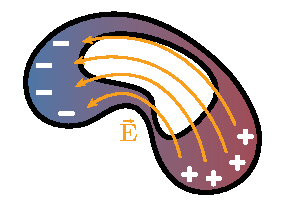
\includegraphics[width=0.4\textwidth]{images/chp2gaussnosimm.pdf}
	\end{center}
	Qui il flusso attraverso la superficie interna è nullo perché ciò che entra esce, ma il campo elettrico \textit{non} è nullo!
\end{attention}
\paragraph{Filo carico rettilineo (infinito)}
	Si consideri un filo rettilineo infinito con densità lineare costante $\lambda$. Per semplicità, poniamo il sistema di riferimento in modo che il filo carico sia lungo l'asse $z$. Poniamo un cilindro attorno al filo in modo che il filo passi per l'asse del cilindro.\\
	\begin{minipage}{0.29\textwidth}
		\begin{center}
			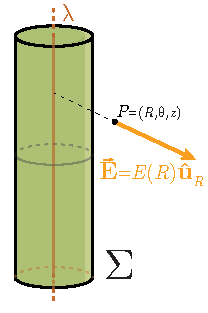
\includegraphics[width=1\textwidth]{images/chp2filoinfinito.pdf}
		\end{center}		% https://betterexplained.com/articles/flux/
	\end{minipage}\hspace{10pt}
	\begin{minipage}{0.7\textwidth}
		Data l'evidente simmetria cilindrica del sistema usiamo, per motivi che dovrebbero essere oramai chiari, le coordinate cilindriche:
		\begin{equation*}
			\begin{cases}
				x=R\cos\theta\\
				y=R\sin\theta\\
				z=z
			\end{cases}
		\end{equation*}
		Oltre ad essere un sistema di riferimento, fissato $R$ abbiamo una parametrizzazione del cilindro di raggio $R$. Ora, ci è già noto che in questo sistema di riferimento il campo elettrostatico dipende esclusivamente dalla \textit{coordinata radiale} e ha direzione radiale, ossia $\vba{E}=E(R)\vbh{u}_R$.
	\end{minipage}\\
Per come abbiamo posto il cilindro $\Sigma$, il versore normale alla superficie laterale coincide con quello radiale delle coordinate cilindriche, pertanto
\begin{equation*}
	\Phi_{\Sigma}(\vba{E})=\int_{\Sigma}\vba{E}\cdot\vbh{u}_nd\Sigma=\int_{\Sigma}\vba{E}\cdot\vbh{u}_Rd\Sigma=\int_{\Sigma} E(R)\vbh{u}_R\vdot\vbh{u}_Rd\Sigma=E(R)\int_{\Sigma} d\Sigma\squarequal
\end{equation*}
dove l'ultimo passaggio è lecito in quanto sulla superficie del cilindro il raggio è fissato e quindi anche $E(R)$ è costante.\\
Dato che l'elemento di area è dato da $d\Sigma=d\Phi dz$, si ha
\begin{equation*}
	\squarequal\lim_{L\to+\infty}2\pi R L E(R)
\end{equation*}
Per la legge di Gauss,
\begin{equation*}
	\Phi_{\Sigma}(\vba{E})=\frac{q}{\epsilon_0}=\frac{\lambda L}{\epsilon_0}
\end{equation*}
dove $\lambda$ è la densità lineare di carica; per ottenere il flusso per il filo infinito ci basterebbe mandare $L$ all'infinito. Eguagliando i due flussi ottenuti si ricava che
\begin{equation*}
	2\pi R\Ccancel[red]{L}E(R)=\frac{\lambda \Ccancel[red]{L}}{\epsilon_0}
\end{equation*}
e quindi
\begin{equation}
	\vba{E}(R)=\frac{\lambda}{2\pi\epsilon_0 R}
\end{equation}
\paragraph{Superficie piana carica infinita}
Si consideri una superficie piana $\Sigma$ con densità superficiale costante $\sigma$. Per semplicità, poniamo il sistema di riferimento in modo che la superficie coincida con il piano $x=0$. Come per il caso del filo carico rettilineo, consideriamo un cilindro, questa volta che interseca la superficie ortogonalmente e posto in maniera che le basi siano alla stessa distanza dal piano.\\
\begin{minipage}{0.43\textwidth}
	\begin{center}
		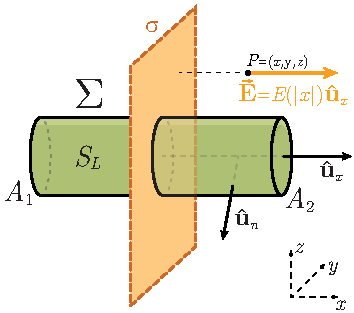
\includegraphics[width=1\textwidth]{images/chp2superficieinfinita.pdf}
	\end{center}		% https://betterexplained.com/articles/flux/
\end{minipage}\hspace{10pt}
\begin{minipage}{0.56\textwidth}
	Ci è già noto che il campo elettrostatico dipende esclusivamente dalla coordinata perpendicolare al piano, cioè $x$, e ha direzione $\vbh{u}_x$. In particolare, si osservi che da facce opposte del piano il versore normale $u_n=u_x$ cambia verso e quindi cambia verso anche il campo elettrostatico:
	\begin{equation*}
		\vba{E}=
		\begin{cases}
			E(\abs{x})\vbh{u}_x&\text{se}\ x>0\\
			-E(\abs{x})\vbh{u}_x&\text{se}\ x<0
		\end{cases}
	\end{equation*}
	Il flusso tramite il cilindro $\Sigma$ si può scindere in tre componenti: i due flussi $\Phi_{A_1}$ e $\Phi_{A_2}$ attraverso le basi e il flusso $\Phi_{SL}$ attraverso la superficie laterale.
\end{minipage}\\
Tuttavia, poiché la superficie laterale è sempre ortogonale al campo, quest'ultima componente è nulla; inoltre, si ha che il campi esce sempre dalle basi, pertanto i flussi saranno positivi e, per questioni di simmetria, coincidono:
\begin{equation}
	\Phi_{A_1}=\Phi_{A_2}
\end{equation}
Pertanto,
\begin{equation*}
	\Phi_{\Sigma}(\vba{E})=2\int_A E(\abs{x})d\Sigma=2 E(\abs{x})\int_{A_1}d\Sigma=2E(\abs{x})A_1
\end{equation*}
Ricordando che la densità di carica superficiale $\sigma$ è costante, la carica interna al cilindro è data da
\begin{equation*}
	q=\sigma A_1
\end{equation*}
Per la legge di Gauss si ha
\begin{equation*}
	\Phi_{\Sigma}=\frac{\sigma A_1}{\epsilon_0}
\end{equation*}
Eguagliando i due flussi ottenuti si ricava che
\begin{equation*}
	2\Ccancel[red]{A_1}E(\abs{x})=\frac{\sigma \Ccancel[red]{A_1}}{\epsilon_0}
\end{equation*}
e quindi
\begin{equation}
	\vba{E}(\abs{x})=\frac{\sigma}{2\epsilon_0}\vbh{u}_x
\end{equation}
\paragraph{Sfera uniformemente carica}
Si consideri una palla sferica di raggio $R$ con densità volumica costante $\rho$. Per semplicità, poniamo il sistema di riferimento in modo che l'origine coincida con il centro della sfera. Come superficie $\Sigma$ per calcolare il flusso scelgo una sfera di raggio $r$ centrata anch'essa nell'origine.
Ci è già noto che il campo elettrostatico dipende esclusivamente dalla coordinata radiale e ha direzione radiale, ossia $\vba{E}=E(r)\vbh{u}_r$. Il versore normale alla superficie $\Sigma$ è $\vbh{u}_n=\vbh{u}_r$.
A questo punto distinguiamo il calcolo quando la superficie sferica ha raggio maggiore della palla ($r>R$) o quando ha raggio minore ($r<R$).
\subparagraph{Il caso esterno: $r>R$}~\\
\begin{minipage}{0.45\textwidth}
	\begin{center}
		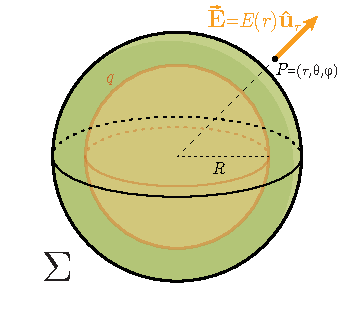
\includegraphics[width=1\textwidth]{images/chp2sferacarica1.pdf}
	\end{center}
\end{minipage}\hspace{5pt}
\begin{minipage}{0.54\textwidth}
	In questo caso la superficie sferica \textit{contiene} la sfera uniformemente carica. Il flusso dunque è
	\begin{equation*}
		\Phi_{\Sigma}(\vba{E})=\int E(r)d\Sigma=E(r)4\pi r^2
	\end{equation*}
	dato che $E(r)$ è costante sulla sfera di raggio $r$.
	La superficie sferica contiene \textit{tutta} la carica della palla al suo interno, quindi per la legge di Gauss
	\begin{equation*}
		\Phi_{\Sigma}(\vba{E})=\frac{q}{\epsilon_0}=\frac{4 \pi R^3\rho}{3\epsilon_0}
	\end{equation*}
	e quindi
	\begin{equation}
		\vba{E}(r)=\frac{\rho R^3}{3\epsilon_0r^2}\vbh{u}_r=\frac{q}{4\pi\epsilon_0 r^2}\vbh{u}_r
	\end{equation}
\end{minipage}\\
\begin{observe}
	Una qualunque distribuzione di carica a simmetria \textit{sferica} dipendente dalla distanza radiale, ossia $\rho(x,y,z)=\rho(r)$, genera al suo esterno un campo uguale a quello di una carica puntiforme.
\end{observe}
\subparagraph{Il caso interno: $r<R$}~\\
\begin{minipage}{0.45\textwidth}
	\begin{center}
		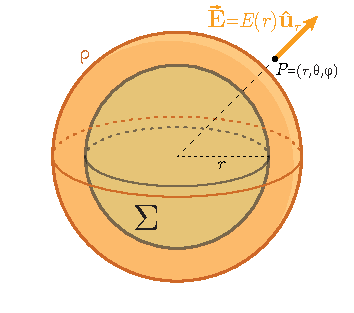
\includegraphics[width=1\textwidth]{images/chp2sferacarica2.pdf}
	\end{center}
\end{minipage}\hspace{5pt}
\begin{minipage}{0.54\textwidth}
	In questo caso la superficie sferica contiene al suo interno solo \textit{una parte} della carica complessiva:
	\begin{equation*}
		q_{int}=\frac{4}{3}\pi r^3\rho
	\end{equation*}
	Se il flusso, calcolato secondo la definizione, non cambia espressione (ma valore sì!)...
	\begin{equation*}
		\Phi_{\Sigma}(\vba{E})=E(r)4\pi r^2
	\end{equation*}
	... quello per la legge di Gauss diventa
	\begin{equation*}
		\Phi_{\Sigma}(\vba{E})=\frac{q_{int}}{\epsilon_0}=\frac{4 \pi r^3\rho}{3\epsilon_0}
	\end{equation*}
	e quindi
	\begin{equation}
		\vba{E}(r)=\frac{q_{int}}{4\pi\epsilon_0 r^2}\vbh{u}_r=\frac{\rho r}{3\epsilon_0}\vbh{u}_r
	\end{equation}
\end{minipage}\\
Riassumendo, il campo elettrico generato da una sfera uniformemente carica di raggio $R$ a distanza $r$ dall'origine è
\begin{equation}
	\vba{E}(r)=\begin{cases}
		\displaystyle\frac{\rho r}{3\epsilon_0}\vbh{u}_r&\text{se}\ r< R\\
		\displaystyle\frac{q}{4\pi\epsilon_0 r^2}\vbh{u}_r=\frac{\rho R^3}{3\epsilon_0r^2}\vbh{u}_r &\text{se}\ r> R
	\end{cases}
\end{equation}
\begin{center}
	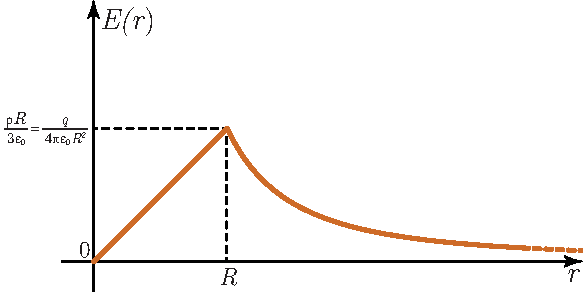
\includegraphics[width=0.75\textwidth]{images/chp2sferagraf1.pdf}
\end{center}
Come già detto, esiste un \textit{potenziale} $V$ tale per cui $\vba{E}=-\grad{V}$. Poiché il campo dipende esclusivamente dalla coordinata radiale, tale relazione si trasforma in
\begin{equation*}
	E(r)=-\pdv{V}{r}
\end{equation*}
da cui
\begin{equation*}
	V(r)=-\int E(r)dr+A
\end{equation*}
dove $A$ è una costante che dipende dalle \textit{condizioni al contorno} di natura fisica. Lasciando tempo alle opportune spiegazioni, per ora ci basti sapere che il \textit{limite all'infinito} del potenziale si pone in generale \textit{nullo}\footnote{Nel \autoref{chap:PotenzialeElettrico}, a pag. \pageref{CondizionialContornoPot} si può trovare la motivazione di ciò.} e che il potenziale è un campo scalare \textit{continuo}\footnote{Nel \autoref{chap:PotenzialeElettrico}, a pag. \pageref{PotenzialeContinuo} si può trovare la motivazione di ciò.}. Integrando le equazioni di campo ottenute ricaviamo
\begin{equation*}
	V(r)=\begin{cases}
		\displaystyle-\frac{\rho r^2}{6\epsilon_0} + A&\text{se}\ r< R\\
		\displaystyle\frac{q}{4\pi\epsilon_0 r} + B=\frac{\rho R^3}{3\epsilon_0r} + B&\text{se}\ r> R
	\end{cases}
\end{equation*}
con $A$ e $B$ opportune costanti. Imponiamo nella seconda equazione il potenziale all'infinito ($r\to+\infty$) nullo - dato che è quella riguardante il sistema a grandi distanze; è immediato trovare che $B=0$. Dalla condizione di continuità invece, il potenziale sul bordo della sfera deve essere uguale ‘‘visto'' dall'\textit{interno} e dall'\textit{esterno}, ossia
\begin{equation*}
	\frac{\rho R^3}{3\epsilon_0R}=-\frac{\rho R^2}{6\epsilon_0} + A
\end{equation*}
Con pochi passi algebrici troviamo
\begin{equation*}
	A=\frac{\rho R^2}{2\epsilon_0}
\end{equation*}
Riassumendo, il potenziale del campo elettrico generato da una sfera uniformemente carica di raggio $R$ a distanza $r$ dall'origine è
\begin{equation}
	V(r)=\begin{cases}
		\displaystyle-\frac{\rho r^2}{6\epsilon_0} + \frac{\rho R^2}{2\epsilon_0}&\text{se}\ r< R\\
		\displaystyle\frac{q}{4\pi\epsilon_0 r} + B=\frac{\rho R^3}{3\epsilon_0r} + B&\text{se}\ r> R
	\end{cases}
\end{equation}
\begin{center}
	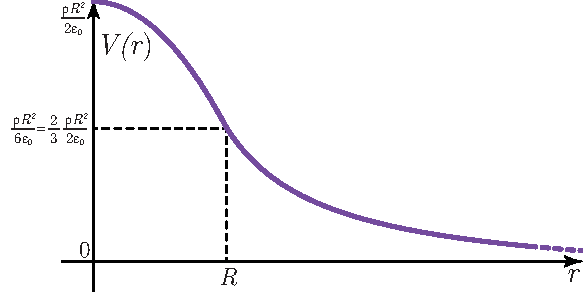
\includegraphics[width=0.75\textwidth]{images/chp2sferagraf2.pdf}
\end{center}
\begin{observe}
	Poiché il sistema ha una dimensione radiale \textit{finita}, si ha come conseguenza la \textit{diminuzione continua} del campo fino all'\textit{annullamento nel campo} nel centro della distribuzione: in questo modo si evita la divergenza all'infinito che si ha con il campo della \textit{carica puntiforme}, oggetto che \textit{fisicamente} è \textit{irrealizzabile} nella teoria classica dell'elettromagnetismo.
\end{observe}
\section{Equilibrio in un campo elettrostatico}
% https://physics.stackexchange.com/questions/190066/why-cant-charge-be-in-a-stable-equilibrium-in-electrostatic-field#:~:text=There%20are%20no%20points%20of,the%20field%20must%20be%20zero.
% https://diego.assencio.com/?index=bc04395b103021d338b4e30a061bfc74
\begin{define}[Equilibrio stabile]
	Un punto $P$ è di \textbf{equilibrio stabile}\index{equilibrio!stabile} per un corpo puntiforme se per un qualsiasi spostamento, piccolo a piacere, da tale posizione esistono forze che riportano l'oggetto nella posizione originale.
\end{define}
\begin{define}[Equilibrio instabile]
	Un punto $P$ è di \textbf{equilibrio instabile}\index{equilibrio!instabile} per un corpo puntiforme se esistono spostamenti, piccolo a piacere, da tale posizione esistono forze che riportano l'oggetto nella posizione originale.
\end{define}
Consideriamo delle \textit{sorgenti} fisse (continue o discrete che siano, \textit{non} cambia) nel vuoto e sia $\vba{E}(\vba{r})$ il campo elettrico generato da queste cariche. Esistono dei punti tali per cui, se poniamo una carica $q$ lì, essa rimarrà in equilibrio stabile?\\
La risposta è \textbf{no} e ce lo dice il \textbf{teorema di Earnshaw}.
\begin{theorema}[Teorema di Earnshaw]\index{teorema!di Earnshaw}
	Una collezione di cariche puntuali non possono essere mantenute in una configurazione di equilibrio stabile soltanto dall'interazione elettrostatica delle cariche con un campo elettrico.
\end{theorema}
In questa dimostrazione assumiamo che la carica sia positiva ($q>0$), ma la dimostrazione è \textit{mutatis mutandis} la stessa per $q<0$.
\begin{observe}
	La carica nella dimostrazione si suppone essere una \textbf{carica di prova}, e quindi il campo generato dalla carica $q$ è trascurabile.
\end{observe}
\begin{demonstration}
	Supponiamo che la carica, immersa nel campo elettrico e non soggetta ad altre forze, è in equilibrio stabile in $P=\vba{r}$; ciò significa che:
	\begin{enumerate}
		\item La carica di per sé è ferma; la forza totale agente sulla carica è dunque nulla, e dato che le uniche forze sulla carica in $\vba{r}$ sono le forza di Coulombsi ha
		\begin{equation*}
			\vba{F}(\vba{r})=q\vba{E}(\vba{r})=0\underset{q\neq 0}{\implies}\vba{E}(\vba{r})=0
		\end{equation*}
		\item Per un (piccolo) spostamento $\delta \vba{r}$ attorno a $\vba{r}$, la forza riporta la carica verso il punto $\vba{r}$, cioè la forza
		\begin{equation*}
			\vba{F}(\vba{r}+\delta\vba{r})=q\vba{E}(\vba{r}+\delta\vba{r})
		\end{equation*}
		deve puntare verso $\vba{r}$.\\
		\begin{minipage}{0.35\textwidth}
			\begin{center}
				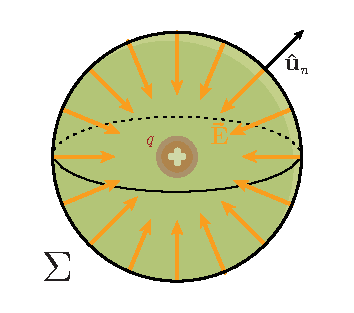
\includegraphics[width=1\textwidth]{images/chp2earnshaw.pdf}
			\end{center}
		\end{minipage}\hspace{5pt}
		\begin{minipage}{0.54\textwidth}
			Consideriamo una superficie chiusa (arbitrariamente piccola) attorno alla carica.
			Per quanto abbiamo detto, in un qualunque suo punto la forza di Coulomb in tal punto deve essere diretta verso $P=\vba{r}$. Pertanto, se il campo è entrante la superficie, il flusso tramite la superficie è negativo...
			\begin{equation}
				\Phi{\Sigma}(\vba{E})<0
			\end{equation}
		\end{minipage}\\
		... ma possiamo applicare la legge di Gauss per ricavare il valore del flusso tramite tale superficie, tuttavia si avrebbe
		\begin{equation*}
			\Phi{\Sigma}(\vba{E})=\frac{q}{\epsilon_0}<0\implies q<0
		\end{equation*}
		il che è un assurdo! Segue che non ci può essere equilibrio elettrostatico stabile.\qedhere
	\end{enumerate}
\end{demonstration}
L'unica possibilità di avere una carica in equilibrio stabile è se si trovasse esattamente nello stesso punto di un'altra carica $Q$ di segno opposto e quantità di carica maggiore. Infatti, in tal caso qualunque superficie, piccolo a piacere, scegliamo attorno al punto di equilibrio si avrà sempre flusso pari a
\begin{equation*}
	\Phi_{\Sigma}(\vba{E})=\frac{q+Q}{\epsilon_0}
\end{equation*}
per la legge di Gauss; questa volta non si ha alcun assurdo, dato che il campo elettrico è entrante e quindi il flusso è negativo e, se $\abs{Q}>\abs{q}$, allora anche il flusso secondo Gauss è negativo.
\begin{digression}
	Da quanto detto, un sistema di cariche libere \textit{dello stesso segno} non potrà ai restare in equilibrio stabile spontaneamente, ma necessariamente occorrono altre forze per vincolare le cariche.
	
	Una conseguenza di ciò è che il modello dell'atomo di Rutherford \textit{non} è stabile, essendo basato su una distribuzione fissata di cariche: nel \textit{nucleo atomico} non ci potrebbe essere più di un protone senza compromettere la stabilità del nucleo! È grazie all'interazione \textit{nucleare forte} che, essendo particolarmente forte a distanze microscopiche, i protoni superano la repulsione elettrostatica tra di loro e permettono la stabilità dell'atomo.
\end{digression}
%TODO: aggiungere